\documentclass[11pt]{article}
%---- defitions ----
\def\Author{Andreas Bock, bock@andreasbock.dk\\
Johan Astborg, joastbg@gmail.com\\\\
Supervisors:\\
Jost Berthold, jb.diku@gmail.com\\
Sinan Gabel, sinan.gabel@gmail.com
}
%\def\Title{\bf Project Synopsis\\ HQL - \textsc{Hiperfit} Quant Library}
\def\Title{\bf HQL - \textsc{Hiperfit} Quant Library\\ {\Large Project Synopsis}}
% <Add more defitions here>
%-------------------

%---- packages ----
\usepackage[]{amsmath}
\usepackage[english]{babel}
\usepackage[utf8]{inputenc}
\usepackage{graphicx}
\usepackage{moreverb}
\usepackage{hyperref}
\usepackage{color}
\usepackage{listings}

%---- settings ----
\topmargin=-1.1in % start text higher on page
\textheight=695pt
\usepackage[T1]{fontenc} % font
\setlength{\parindent}{0in}
\definecolor{lightgray}{rgb}{0.9,0.9,0.9}

\newenvironment{filecode}[1][]
{\minipage{\linewidth}
\lstset{basicstyle=\ttfamily\footnotesize,frame=single,
numberstyle=\small\color{black},keywordstyle=\color{black},commentstyle=\color{black},stringstyle=\color{black},tabsize=2,backgroundcolor=\color{lightgray},language=Haskell,#1}}
{\endminipage}
%-------------------

\begin{document}
\title{\Title}
\author{\Author}
\date{\today}
\maketitle

\begin{abstract}

% Something about how pricing is done now, and what we will do

\end{abstract}

\section*{Introduction}

Our everyday lives becoming increasingly dependent on IT, and as a result, software
errors are manifold. The financial sector has a particular low tolerance, as erroneous
software may have dire consequences in the form of massive monetary loss.\\
Human brokers are replaced by web-based services, and traders are now joined by
colocated machines that perform high-frequency trading.

% Open source -> do banks want a uniform quant platform..? cite if possible
%Things have changed and new requirements and technologies are pushing the needs
%of a redesign in a more open language. Also, insights into source code and the
%details behind an implementation is something the market asks for.

% Algorithms
These tools may help increase competitiveness and profits, but emphasize the
importance of correct code.

Automated algorithmic trading systems are considered to have lower operational risk due to the lack
of human contact, but require software correctness to work. An otherwise feasible
trading model could wreak havoc on markets because of a software error.

% Safeguards are also compromised
Further, brokerages and exchanges attempt to lower operational risk by implementing
safeguards to make it difficult for human error to affect markets (e.g. fat-fingering
trades\footnote{Human error causing larges trades to be made that create sudden
imbalances in the markets.}). Albeit thoroughly tested, bugs are ubiquitous and these
safeguards may be just as prone to them. 

% Legislation, cite new Danish regulations?
The financial crisis of 2008 also caused legislators to take a more conservative
stance on risk, as the collapse on Lehman Brothers reverberated throughout
the world's economies.
Consequently, financial institutions' risk management tools must become more
sophisticated, putting stress on the quality of the software.

By designing and building correct and safe software we may hope to eliminate some
of the unnecessary risk in financial modelling.

\section*{Problem Statement}

In this project we will design the software architecture for a Haskell library for quantitative finance.
The desired functionality is modeled after an existing Mathematica library {\tt DerivativesExpert}, which
we will re-engineer into Haskell.
The main objective is to use the Haskell programming language for design and architecture and reach a proof-of-concept level.
The project is limited to research within the HIPERFIT research center.

\section*{Elaboration}

% TODO Mention Quantlib
In finance, a portfolio is a number of positions such as positions in equities, bonds and other
types of financial instruments. The present value of such a collection can be computed through
discounting to reflect the theoretical value they would have if they existed today. This allows
investors to evaluate if their resources could yield higher returns elsewhere.
Financial instruments are priced differently, some using closed-form functions and
others relying on stochastic simulation. In this project, we'll mainly work with bonds and
time value of money.\\

Functional languages lend themselves well to the domain of finance due
to several reasons. Firstly, functions are first-class citizens, and programs are constructed
from functions entirely. Because of the mathematical nature of finance, a functional
language is preferable and makes it easier to write and test mathematical expressions.\\

Further, Haskell is a pure language meaning that a function will always return the same value
if given the same input\footnote{with exceptions such as {\tt IO}}. This makes it ideal for
financial computations where we want to be certain our computations are not changed by some
global state.\\

Combining Haskell's purity with its modularity, we can also allow for users to `glue`
together functions without the worry that, for instance, the first function call has changed
a value through a pointer. Function composition in this manner does not mean we
take a penalty performance-wise, since the non-strictness of the language  means that
we only evaluate the things we need.\\

Additionally, Haskell is a statically typed language with type inference. As such, 
types and type classes make up a large portion of the language design. Statically typed languages have the
advantage of discovering many errors at compile time, and the type class system enables us to overload
functionality in our programs based on our types. This is a very desirable feature, as we want our financial products

A proof-of-concept example of the inheritance relation that we want our library
to feature is shown in listing \ref{lst:inh}.

\begin{filecode}[caption=Inheritance relations using type classes, label={lst:inh}]
\lstinputlisting{Example.hs}
\end{filecode}\\

Finally, functional languages can easily preserve the inherent parallelism of computations 
making them ideal for performance-critical tasks such as pricing financial products or
computing risk.\\

In summary, our focus will be on exploring how Haskell's advanced language features can be used
to ensure safe and correct code, without compromising a good extendable software architecture.

% Mathematica "port"
%Finally, the library will be heavily influenced by the {\tt DerivativesExpert} package developed by Sinan Gabel for the \emph{Mathematica} software\cite{Mathematica:DerivativesExpert}.

\section*{Learning Goals}

Learning goals and objectives:

\begin{enumerate}
\item The student will be able to design and implement medium to large scale software systems in a functional language. % arch
%\item The student will be able to identify and use features of a functional language to enforce the necessary correctness needed in financial computing. % correctness
\item The students will be able to describe the concepts of financial valuation and its relevance to portfolio management. % finance
\item The students will be able to develop a sustainable and extendable prototype Haskell library for pricing common financial products. % concrete result
\item To translate the functionality of existing software and re-engineer it in a functional language.
\end{enumerate}

\section*{Limitations}

% 1) Not a fully-fledged library like DE or Quantlib
Firstly, we will not expect to produce a fully-fledged library like {\tt DerivativesExpert} or Quantlib\cite{Ame2003}.
% 2) Benchmarking or comparisons (?)
Secondly, and partly due to the point above, we will not perform an in-depth survey
comparing the result of our project with similar ones such as the aforemetioned libraries.

% 3)

The project is mainly limited by time, a constraint derived from the project course 
format (one block lasting approximately 9 weeks).
The scope has been narrowed to fit the size of the project, and will mainly include
pricing functionality for bonds specified in the {\tt DerivativesExpert} package.

\section*{Possible additions}

\section*{Schedule}

%% Use milestones here instead?

Below is our approximate schedule over the course of the project:\\

\begin{figure}[h!]
\begin{center}
%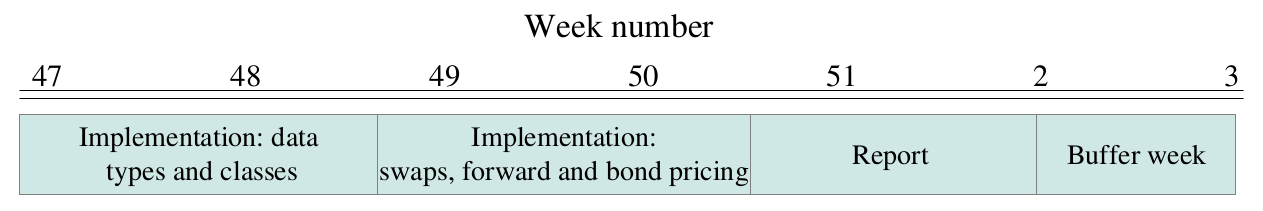
\includegraphics[bb = 0 0 1302 348, scale=0.275]{schedule.png}
\end{center}
\end{figure}

% REFERENCES
\bibliographystyle{abbrv}
%\addcontentsline{toc}{section}{References}
\bibliography{hql}

\end{document}
